% Created 2021-09-27 Mon 19:31
% Intended LaTeX compiler: pdflatex
\documentclass[11pt]{article}
\usepackage[utf8]{inputenc}
\usepackage[T1]{fontenc}
\usepackage{graphicx}
\usepackage{grffile}
\usepackage{longtable}
\usepackage{wrapfig}
\usepackage{rotating}
\usepackage[normalem]{ulem}
\usepackage{amsmath}
\usepackage{textcomp}
\usepackage{amssymb}
\usepackage{capt-of}
\usepackage{hyperref}
\usepackage[hidelinks]{hyperref}
\usepackage{minted}
\usemintedstyle{lovelace}
\date{\today}
\title{}
\hypersetup{
 pdfauthor={},
 pdftitle={},
 pdfkeywords={},
 pdfsubject={},
 pdfcreator={Emacs 27.2 (Org mode 9.4.4)}, 
 pdflang={English}}
\begin{document}

\tableofcontents


\section{Comandos utilizados}
\label{sec:org874db36}
\subsection{Classe do documento (comando)}
\label{sec:orgc639ab2}
\begin{minted}[fontsize=\scriptsize,autogobble=false,frame=lines,framesep=4pt,linenos=false]{latex}
\documentclass[bigger]{beamer}
\end{minted}

\subsection{Importação de pacotes (comando)}
\label{sec:orgd71a6cf}

Para qualquer pacote listado no \url{https://www.ctan.org/}, basta chamarmos
o seguinte comando para incorporá-lo no documento em mãos.

\begin{minted}[fontsize=\scriptsize,autogobble=false,frame=lines,framesep=4pt,linenos=false]{latex}
\usepackage{<nome-do-pacote>}
\end{minted}

\subsubsection{Estilizações de um pacote}
\label{sec:orgd8521ed}

\begin{enumerate}
\item Exemplo \texttt{tcolorbox}
\label{sec:orgebd9e0f}
Alguns pacotes possuem estilização interna ao pacote. Por exemplo,
\texttt{tcolorbox}, um pacote utilizado para estilizar blocos e tabelas, pode
requerir a chamada de um "subpacote" adicional.

Exemplo:
Na documentação, é dito, para importação de bibliotecas extras, dentro
de tcolorbox,
\url{http://mirrors.ctan.org/macros/latex/contrib/tcolorbox/tcolorbox.pdf}
É dito, utilize essa sintaxe.

\begin{minted}[fontsize=\scriptsize,autogobble=false,frame=lines,framesep=4pt,linenos=false]{latex}
\tcbuselibrary{⟨key list⟩}
\end{minted}

Todas as opções:

\href{img/libraries-tcolobox.png}{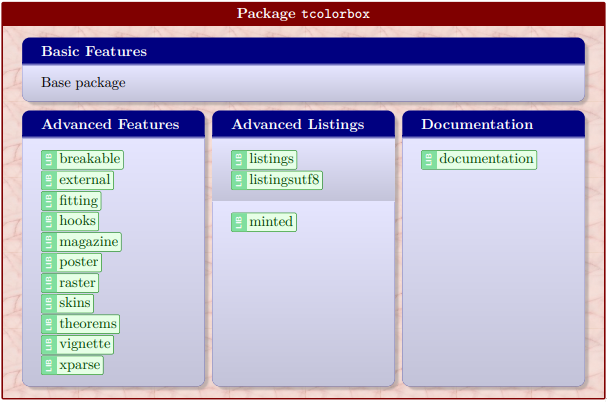
\includegraphics[width=0.5\textwidth]{/home/buddhilw/PP/LaTeX/SEMEF-minicurso/Apres1/img/libraries-tcolobox.png}}

\item Caso de uso, na apresentação:
\label{sec:org358e6a0}

No \texttt{preâmbulo}, chamei o pacote e biblioteca
\begin{minted}[fontsize=\scriptsize,autogobble=false,frame=lines,framesep=4pt,linenos=false]{latex}
\usepackage{tcolorbox}
\tcbuselibrary{skins}
\end{minted}

Adaptei um exemplo da documentação,
\begin{minted}[fontsize=\scriptsize,autogobble=false,frame=lines,framesep=4pt,linenos=false]{latex}
\newenvironment{modern-quote}{\begin{itemize}}{\end{itemize}}
\tcolorboxenvironment{modern-quote}{blanker,
  before skip=6pt,
  after skip=6pt,
  borderline west={3mm}{0pt}{red}}
\end{minted}

Por fim, para chamar o novo ambiente no documento, temos,
\begin{minted}[fontsize=\scriptsize,autogobble=false,frame=lines,framesep=4pt,linenos=false]{latex}
\begin{modern-quote}
"Don't give up on your dreams, keep on sleeping."
\end{modern-quote}
\end{minted}

\begin{enumerate}
\item Renderização:
\label{sec:org7580c26}

\href{img/modern-quote.png}{
\includegraphics[width=0.4\textwidth]{/home/buddhilw/PP/LaTeX/SEMEF-minicurso/Apres1/img/modern-quote.png}}
\end{enumerate}
\end{enumerate}

\subsubsection{Todos pacotes utilizados na apresentação, com suas opções e bibliotecas.}
\label{sec:org8cce462}
\begin{minted}[fontsize=\scriptsize,autogobble=false,frame=lines,framesep=4pt,linenos=false]{latex}
\usepackage[utf8]{inputenc}
\usepackage[T1]{fontenc}
\usepackage{graphicx}
\usepackage{grffile}
\usepackage{longtable}
\usepackage{wrapfig}
\usepackage{rotating}
\usepackage[normalem]{ulem}
\usepackage{amsmath}
\usepackage{textcomp}
\usepackage{amssymb}
\usepackage{capt-of}
\usepackage{hyperref}
\author[Branquinho]{Pedro Gomes Branquinho \\ \text{\scriptsize{pedro.branquinho@usp.br}}}
\date[EEL-USP]{\scriptsize{Mini-curso de \LaTeX} \\ Universidade de São Paulo - DEMAR}
\usepackage{pifont}
\usepackage{verbatim}
\makeatletter
\def\verbatim@font{\scriptsize\ttfamily}
\makeatother
\logo{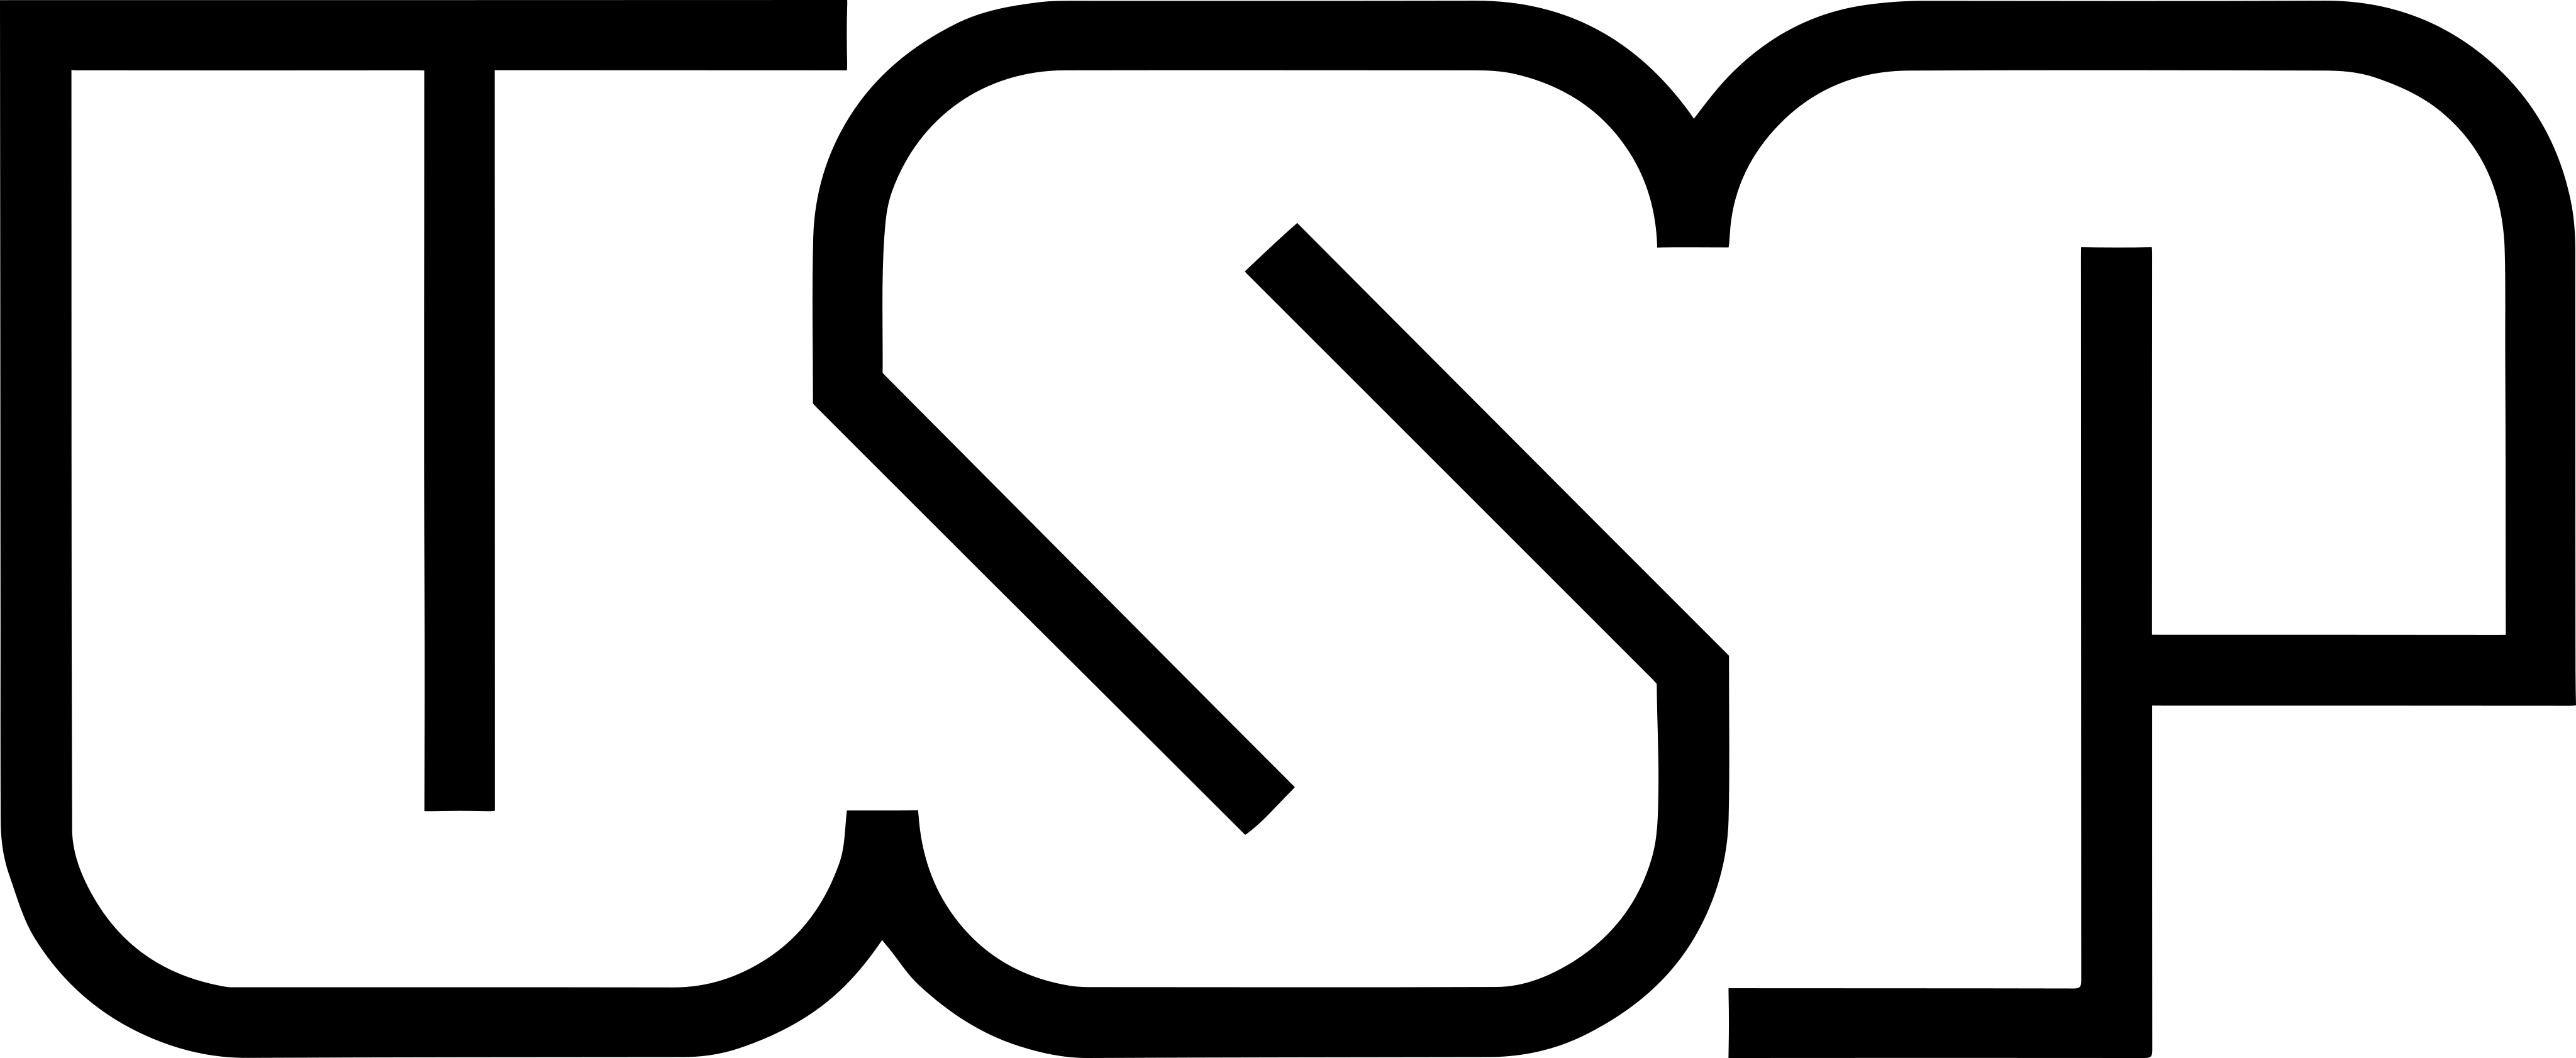
\includegraphics[height=0.5cm]{./img/usp-logo-1}}
\AtBeginSubsection[]{\begin{frame}\frametitle{Table of Contents}
    \tableofcontents[currentsection,currentsubsection]
  \end{frame}}
\usepackage{tikz}
\usetikzlibrary{arrows.meta}
\usetikzlibrary{positioning}
\usepackage{tcolorbox}
\tcbuselibrary{skins}
\usepackage{minted}
\usemintedstyle{lovelace}
\newenvironment{modern-quote}{\begin{itemize}}{\end{itemize}}
\tcolorboxenvironment{modern-quote}{blanker,before skip=6pt,after skip=6pt, borderline west={3mm}{0pt}{red}}
{\usebackgroundtemplate{
\includegraphics[width=\paperwidth]{./img/TP-opacity-50.jpg}}
  \usetheme[height=20pt]{Hannover}
  \usecolortheme{seahorse}
  \date{  Universidade de São Paulo - DEMAR}
  \title{O \LaTeX{} e suas funcionalidades}
  \setbeamertemplate{itemize item}{\ding{166}}
  \setbeamercolor{item projected}{bg=magenta!90!black,fg=white}
  \setbeamertemplate{enumerate item}[circle]
  \setbeamercolor{block title}{bg=red!30!white,fg=black}
  \hypersetup{
    pdfauthor={},
    pdftitle={O \LaTeX{} e suas funcionalidades},
    pdfkeywords={},
    pdfsubject={},
    pdfcreator={Emacs 27.2 (Org mode 9.4.4)}, 
    pdflang={Portuguese}}
\end{minted}

\subsection{Inicialização de slides (ambiente)}
\label{sec:org4078fff}
\subsubsection{Uso}
\label{sec:org6223350}
\begin{minted}[fontsize=\scriptsize,autogobble=false,frame=lines,framesep=4pt,linenos=false]{latex}
\begin{frame}[label={sec:org03cdf3a},fragile]{Origem de \TeX{} - Knuth (1978)}
  (...)
\end{frame}
\end{minted}

\subsubsection{Renderização}
\label{sec:orgb13ecb0}
\href{img/frame.png}{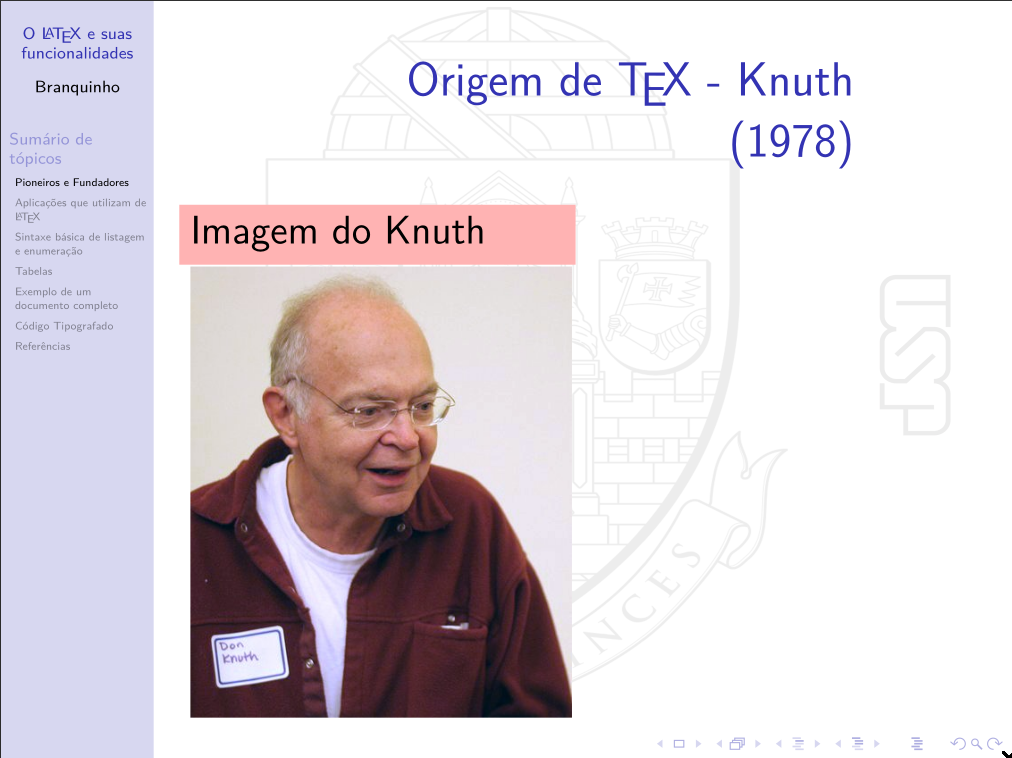
\includegraphics[width=0.3\textwidth]{/home/buddhilw/PP/LaTeX/SEMEF-minicurso/Apres1/img/frame.png}}

\subsection{Compartição de slides em colunas (ambientes)}
\label{sec:org016b584}
\subsubsection{Uso}
\label{sec:org74b0016}

Dentro do ambiente \texttt{frame}, teremos um ambiente \texttt{columns}, o qual pode
ser dividido em diversas colunas unitárias, com  \texttt{column}. Nesse caso,
cada uma ocupou 48\% do espaço disponível para a coluna

\begin{minted}[fontsize=\scriptsize,autogobble=false,frame=lines,framesep=4pt,linenos=false]{latex}
\begin{frame}[label={sec:org03cdf3a},fragile]{Origem de \TeX{} - Knuth (1978)}
  %%%%%% Ambiente interior a um frame
  \begin{columns}

    %%% * Coluna 1
    \begin{column}{0.48\columnwidth}
      (...) % Imagem
    \end{column}

    %%% * Coluna 2
    \begin{column}{0.48\columnwidth} 
      (...) % Código tipografado
    \end{column}

  \end{columns}
  %%%%%% 
\end{frame}
\end{minted}
\subsubsection{Renderização}
\label{sec:orgd4117ef}
\href{img/colunas.png}{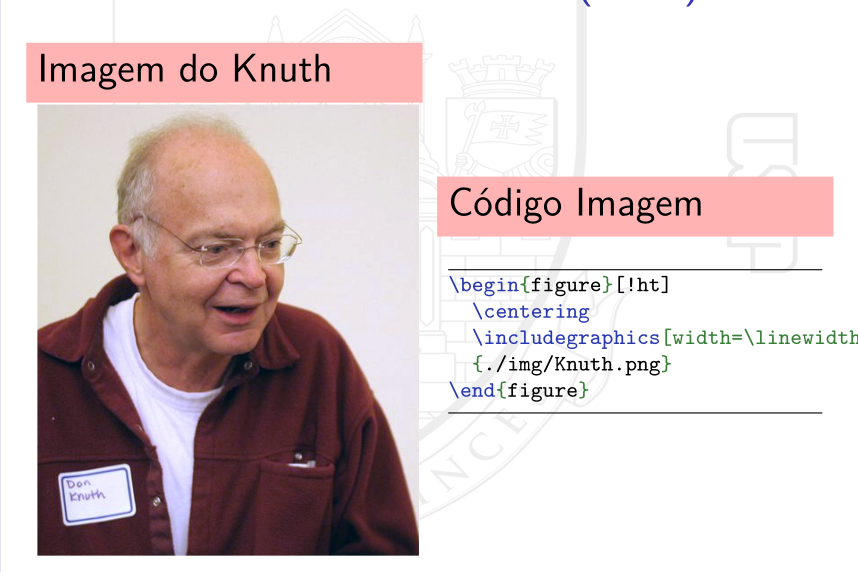
\includegraphics[width=0.5\textwidth]{/home/buddhilw/PP/LaTeX/SEMEF-minicurso/Apres1/img/colunas.png}}

\subsection{Blocos de texto (ambiente)}
\label{sec:org805f744}
No preâmbulo, especificação de fonte preta e fundo rosa claro.
\begin{minted}[fontsize=\scriptsize,autogobble=false,frame=lines,framesep=4pt,linenos=false]{latex}
\setbeamercolor{block title}{bg=red!30!white,fg=black}
\end{minted}

\subsubsection{Exemplo e renderização}
\label{sec:org3c31970}
No corpo do documento
\begin{minted}[fontsize=\scriptsize,autogobble=false,frame=lines,framesep=4pt,linenos=false]{latex}
\begin{block}{\small{~Ille eruditus et sapiens~}}
(...)
\end{block}
\end{minted}

\href{img/titulo-bloco.png}{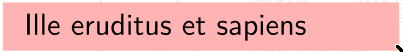
\includegraphics[width=0.3\textwidth]{/home/buddhilw/PP/LaTeX/SEMEF-minicurso/Apres1/img/titulo-bloco.png}}
\subsection{Itemização (ambiente)}
\label{sec:orgde2bed2}
\subsubsection{Customização da itemização}
\label{sec:org4982f11}
No preâmbulo, itens de símbolo ding 166.
\begin{minted}[fontsize=\scriptsize,autogobble=false,frame=lines,framesep=4pt,linenos=false]{latex}
\usepackage{pifont} %Alguns símbolos unicode (dingbats)
\setbeamertemplate{itemize item}{\ding{166}} % Todo itemize será renderizado com esse símbolo 166.
\end{minted}
\begin{enumerate}
\item Uso e renderização
\label{sec:org14ac33b}
Nota: as opções \texttt{[<+->]}, fazem com que os itens apareçam
gradualmente, a cada slide consecutivo.

\begin{minted}[fontsize=\scriptsize,autogobble=false,frame=lines,framesep=4pt,linenos=false]{latex}
\begin{itemize}[<+->]
\item Preview em tempo real.
(...)
\end{itemize}
\end{minted}

\href{img/ding.png}{
\includegraphics[width=0.4\textwidth]{/home/buddhilw/PP/LaTeX/SEMEF-minicurso/Apres1/img/ding.png}}
\end{enumerate}

\subsubsection{Customização do enumerate}
\label{sec:org737bb8f}
No preâmbulo, elementos redondos e rosas.
\begin{minted}[fontsize=\scriptsize,autogobble=false,frame=lines,framesep=4pt,linenos=false]{latex}
\setbeamercolor{item projected}{bg=magenta!90!black,fg=white} % elementos enumerados estilizados (magenta escura)
\setbeamertemplate{enumerate item}[circle] %enumeração com fundo redondo
\end{minted}

\begin{enumerate}
\item Uso e renderização
\label{sec:org15b36f7}
\begin{minted}[fontsize=\scriptsize,autogobble=false,frame=lines,framesep=4pt,linenos=false]{latex}
\begin{enumerate}
\item Primeiro item
\item Segundo item
\end{enumerate}
\end{minted}

\href{img/enumerate.png}{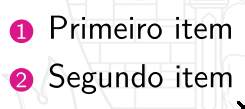
\includegraphics[width=0.2\textwidth]{/home/buddhilw/PP/LaTeX/SEMEF-minicurso/Apres1/img/enumerate.png}}
\end{enumerate}
\subsection{Imagens}
\label{sec:org4386816}
\subsubsection{Uso}
\label{sec:org6203a98}

Dentro de uma \texttt{coluna}, em um \texttt{frame}, temos um \texttt{bloco} com uma
\texttt{imagem}.

\begin{minted}[fontsize=\scriptsize,autogobble=false,frame=lines,framesep=4pt,linenos=false]{latex}
\begin{block}<1->{Imagem Lamport}
  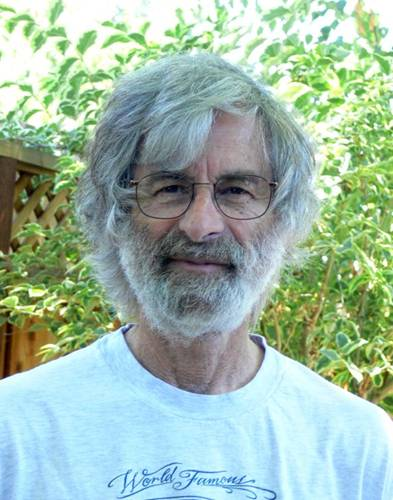
\includegraphics[width=1.02\textwidth]{./img/Leslie_Lamport.jpg}
\end{block}
\end{minted}

\subsubsection{Renderização}
\label{sec:org34e729b}
\href{img/bloco-image.png}{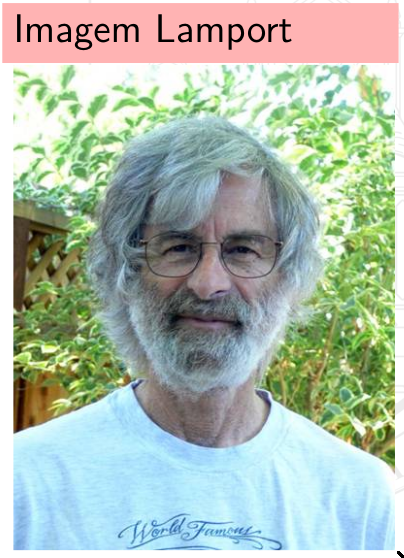
\includegraphics[width=0.3\textwidth]{/home/buddhilw/PP/LaTeX/SEMEF-minicurso/Apres1/img/bloco-image.png}}
\subsection{Equações}
\label{sec:org9d2f5be}
\subsubsection{Uso}
\label{sec:org7756a93}
Em ambientes \texttt{equation}, tipografamos uma equação,
\begin{minted}[fontsize=\scriptsize,autogobble=false,frame=lines,framesep=4pt,linenos=false]{latex}
\begin{equation}
  \begin{aligned}
    \dfrac{\partial{\vec{V}}}{\partial{t}}
    + \vec{V}.\nabla{\vec{V}}
    = - \dfrac{\nabla{p}}{\rho}
    + \nu{}\nabla^2{\vec{V}}
  \end{aligned}
\end{equation}
\end{minted}

\subsubsection{Renderização}
\label{sec:orgbec415c}

\begin{enumerate}
\item Por imagem
\label{sec:org8a66c46}

\href{img/navier.png}{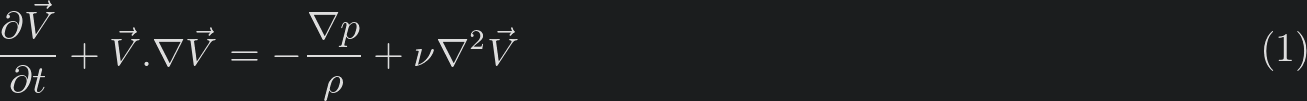
\includegraphics[width=\textwidth]{/home/buddhilw/PP/LaTeX/SEMEF-minicurso/Apres1/img/navier.png}}

\item Por código
\label{sec:orgd82fc8b}

\begin{equation}
  \begin{aligned}
    \dfrac{\partial{\vec{V}}}{\partial{t}}
    + \vec{V}.\nabla{\vec{V}}
    = - \dfrac{\nabla{p}}{\rho}
    + \nu{}\nabla^2{\vec{V}}
  \end{aligned}
\end{equation}
\end{enumerate}
\subsection{Tabelas (ambiente)}
\label{sec:org3a38ea6}
\subsubsection{Uso}
\label{sec:org0d935c2}
Notas:
\begin{itemize}
\item O ambiente pode ser \texttt{tabular} or \texttt{table}
\item \texttt{\textbackslash{}(x=y\textbackslash{})} é equivalente a \texttt{\$x=y\$}. Ou seja, \texttt{\$} e \texttt{\textbackslash{}(} ou \texttt{\textbackslash{})} são intercambiáveis. Porém, não deve os utilizar parcialmente. Isso é, o código \texttt{\$x=y\textbackslash{})} não renderiza corretamente.
\item \texttt{\{lll\}} significa, três elementos por linha, cada um alinhado à esquerda (left).
\item \texttt{\&} são separadores de elementos, por coluna.
\item \texttt{\textbackslash{}\textbackslash{}} quebram linhas
\item \texttt{\textbackslash{}hline} significa uma linha horizontal ``(h[orizontal]line)''
\end{itemize}

\begin{minted}[fontsize=\scriptsize,autogobble=false,frame=lines,framesep=4pt,linenos=false]{latex}
\begin{tabular}{lll}
  \hline
  Coluna 1 & Coluna 2 & Coluna 3\\
  \hline
  \(a_{11}\) & \(a_{12}\) & \(a_{13}\)\\
  \(a_{21}\) & \(a_{22}\) & \(a_{23}\)\\
  Texto 1 & Texto 2 & Texto 3\\
  \hline
\end{tabular}
\end{minted}

Outro exemplo, mas de acordo com as normas ABNT

\begin{minted}[fontsize=\scriptsize,autogobble=false,frame=lines,framesep=4pt,linenos=false]{latex}
\begin{table}[htb]
  \begin{center}

    \ABNTEXfontereduzida

    \caption[<como aparece na lista de tabelas>]{\label{tab:formal} Formatação Tipográfica, modelo de
      tabela genérica}

    \begin{tabular}{m{2.6cm}|m{4.0cm}|m{2.25cm}|m{3.40cm}}
      % \hline
      \textbf{Pretendemos} & \textbf{Temos} & \textbf{Em \LaTeX{}es} & \textbf{Alternativamente}\\
      \hline
      Serif & {\rmfamily\textbf{R}o\textbf{m}ana} & \verb+{\rmfamily}+  & \verb+\textrm{}+ \\
      \hline
      Sans Serif & {\sffamily{\textbf{S}ans Serif\textbf{f}} & \verb+{\sffamily}+  & \verb+\textsf{}+\\
      \hline
      Type Writer & {\ttfamily{\textbf{T}ype Wri\textbf{t}er}}  & \verb+{\ttfamily}+ & \verb+\texttt{}+\\
      \hline
    \end{tabular}
    \legend{Fonte: o autor}

  \end{center}
\end{table}
\end{minted}

Note que temos a estrutura,

\begin{minted}[fontsize=\scriptsize,autogobble=false,frame=lines,framesep=4pt,linenos=false]{latex}
\begin{table}[opções-de-disposição-espacial]
  (texto)
  \begin{tabular}[partições]
    (...)
  \end{tabular}
  (texto)
\end{table}
\end{minted}

\subsubsection{Renderiza}
\label{sec:org03a8ec9}
\begin{enumerate}
\item Por imagem
\label{sec:org9258600}

\href{img/tabela-img.png}{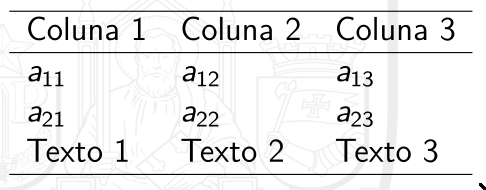
\includegraphics[width=0.5\textwidth]{/home/buddhilw/PP/LaTeX/SEMEF-minicurso/Apres1/img/tabela-img.png}}

\item Por código
\label{sec:orgd5e8a67}
\begin{enumerate}
\item Exemplo 1
\label{sec:orgbd27c4e}

\begin{tabular}{lll}
  \hline
  Coluna 1 & Coluna 2 & Coluna 3\\
  \hline
  \(a_{11}\) & \(a_{12}\) & \(a_{13}\)\\
  \(a_{21}\) & \(a_{22}\) & \(a_{23}\)\\
  Texto 1 & Texto 2 & Texto 3\\
  \hline
\end{tabular}
\item Exemplo 2
\label{sec:org4344899}

\begin{table}[htb]
  \begin{center}

    \ABNTEXfontereduzida

    \caption[<como aparece na lista de tabelas>]{\label{tab:formal} Formatação Tipográfica, modelo de
      tabela genérica}

    \begin{tabular}{|m{2.6cm}|m{4.0cm}|m{2.25cm}|m{3.40cm}}
      \hline
      \textbf{Pretendemos} & \textbf{Temos} & \textbf{Em \LaTeX{}es} & \textbf{Alternativamente}\\
      \hline
      Serif & {\rmfamily\textbf{R}o\textbf{m}ana} & \verb+{\rmfamily}+  & \verb+\textrm{}+ \\
      \hline
      Sans Serif & {\sffamily{\textbf{S}ans Serif\textbf{f}} & \verb+{\sffamily}+  & \verb+\textsf{}+\\
      \hline
      Type Writer & {\ttfamily{\textbf{T}ype Wri\textbf{t}er}}  & \verb+{\ttfamily}+ & \verb+\texttt{}+\\
      \hline
    \end{tabular}
    \legend{Fonte: o autor}

  \end{center}
\end{table}
\end{enumerate}
\end{enumerate}

\section{Vocábulos e notações}
\label{sec:org3962b0e}

\begin{center}
\begin{tabular}{ll}
\hline
Abreviação & Significado\\
\hline
\texttt{bg} & background.\\
\texttt{fg} & foreground.\\
\hline
\end{tabular}
\end{center}

\section{Beamer opçoes estilizaveis}
\label{sec:org03aaff6}
\subsection{Fonte e cor}
\label{sec:org5150e75}
abstract
abstract title
alerted text
author
author in head/foot
author in sidebar
background
background canvas
bibliography entry author
bibliography entry location
bibliography entry note
bibliography entry title
bibliography item
block body
block body alerted
block body example
block title
block title alerted
block title example
button
button border
caption
caption name
date
date in head/foot
date in sidebar
description item
enumerate item
enumerate subitem
enumerate subsubitem
example text
fine separation line
footline
framesubtitle
frametitle
frametitle right
headline
institute
institute in head/foot
institute in sidebar
item
item projected
itemize item
itemize subitem
itemize subsubitem
itemize/enumerate body
itemize/enumerate subbody
itemize/enumerate subsubbody
local structure
logo
lower separation line foot
lower separation line head
math text
math text displayed
math text inlined
middle separation line foot
middle separation line head
mini frame
navigation symbols
navigation symbols dimmed
normal text
normal text in math text
normal text in math text
page number in head/foot
palette primary
palette quaternary
palette secondary
palette sidebar primary
palette sidebar quaternary
palette sidebar secondary
palette sidebar tertiary
palette tertiary
part name
part title
qed symbol
quotation
quote
section in head/foot
section in sidebar
section in sidebar shaded
section in toc
section in toc shaded
section name
section number projected
section title
separation line
sidebar
sidebar left
sidebar right
structure
subitem
subitem projected
subsection in head/foot
subsection in sidebar
subsection in sidebar shaded
subsection in toc
subsection in toc shaded
subsection name
subsection number projected
subsection title
subsubitem
subsubitem projected
subsubsection in head/foot
subsubsection in sidebar
subsubsection in sidebar shaded
subsubsection in toc
subsubsection in toc shaded
subsubsection number projected
subtitle
title
title in head/foot
title in sidebar
titlegraphic
titlelike
upper separation line foot
upper separation line head
verse
\subsection{Transiçoes de slides}
\label{sec:org5797550}
\begin{itemize}
\item Show the slide as if horizontal blinds were pulled away.
\end{itemize}
\texttt{\textbackslash{}transblindshorizontal}
\begin{itemize}
\item Show the slide as if vertical blinds were pulled away.
\end{itemize}
\texttt{\textbackslash{}transblindsvertical}
\begin{itemize}
\item Show the slide by moving to the center from all four sides.
\end{itemize}
\texttt{\textbackslash{}transboxin}
\begin{itemize}
\item Show the slide by showing more and more of a rectangular area that is centered on the slide center
\end{itemize}
\texttt{\textbackslash{}transboxout}
\begin{itemize}
\item Slowly dissolve what was shown before
\end{itemize}
\texttt{\textbackslash{}transdissolve}
\begin{itemize}
\item Glitter sweeps in specified direction
\end{itemize}
\texttt{\textbackslash{}transglitter}
\begin{itemize}
\item Show the slide by sweeping two vertical lines from the sides inward.
\end{itemize}
\texttt{\textbackslash{}transsplitverticalin}
\begin{itemize}
\item Show the slide by sweeping two vertical lines from the center outward.
\end{itemize}
\texttt{\textbackslash{}transsplitverticalout}
\begin{itemize}
\item Show the slide by sweeping two horizontal lines from the sides inward.
\end{itemize}
\texttt{\textbackslash{}transsplithorizontalin}
\begin{itemize}
\item Show the slide by sweeping two horizontal lines from the center outward.
\end{itemize}
\texttt{\textbackslash{}transsplithorizontalout}
\begin{itemize}
\item Sweeps single line in specified direction
\end{itemize}
\texttt{\textbackslash{}transwipe}
\begin{itemize}
\item Show slide specified number of seconds
\end{itemize}
\texttt{\textbackslash{}transduration\{2\}}
\begin{itemize}
\item Show the slide by pushing what was shown before off the screen using the new content.
\end{itemize}
\texttt{\textbackslash{}transpush}
\begin{itemize}
\item Replace the previous slide directly (default behaviour).
\end{itemize}
\texttt{\textbackslash{}transreplace}
\begin{itemize}
\item Show the slide by covering the content that was shown before
\end{itemize}
\texttt{\textbackslash{}transcover}
\end{document}